\documentclass[10pt,a4paper]{article}
\usepackage[utf8]{inputenc}
\usepackage[english]{babel}
\usepackage{amsmath}
\usepackage{hyperref}
\usepackage{graphicx}
\usepackage{tikz}
\usepackage{amsfonts}
\usepackage{amssymb}
\usepackage{qtree}
\usepackage{tikz-qtree}

%\usepackage{xyling}
%\usepackage{xy-picture}

\usepackage{geometry}
\geometry{
	left=2cm,
	right=2cm,
	top=2cm,
	bottom=3cm,
	bindingoffset=5mm
}

\author{Prof. Huson \\
	Script by Sylvia Siegel}
\title{	Pylogeny and Evolution }
\date {WS 2015/ 2016}

\newtheorem {defi}{Definition}[section]
\newtheorem{eg}{Example}[section]

\usetikzlibrary{arrows,automata}

\begin{document}
\maketitle 
\section{Graphs and Trees}
\begin{defi}
Graphs represent relationships. \\
A node represents an object, while edges represent relationships. 

\end{defi}
\begin{eg}{\textbf{Examples in Biology}}
	\begin{itemize}
		\item food webs
\begin{figure}[h"]
	\centering
	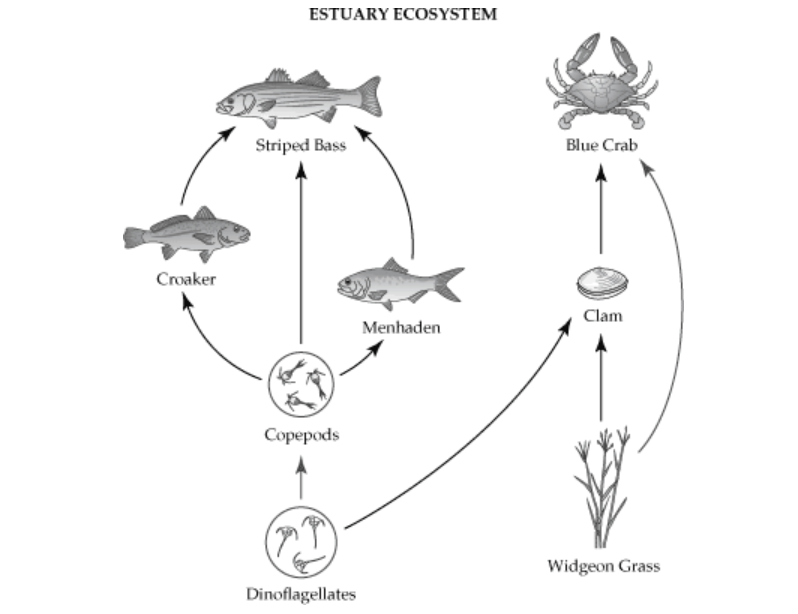
\includegraphics[width = 0.4 \textwidth]{pictures/foodweb}
	\caption[Food web]{
		\centering
		A food web of maritine animals. 
		}
	\label{fig:foodweb}
\end{figure}

\item metabolic pathways 
	\begin{figure} [h!]
		\centering
		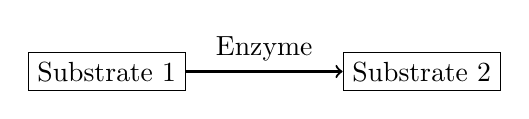
\begin{tikzpicture}
			\node (sub1) at (3,0) [rectangle, draw] {Substrate 1}; 
			\node (sub2) at (7,0) [rectangle, draw] {Substrate 2};
			
			\draw [thick, ->] (sub1) to node [above] {Enzyme} (sub2) ;  
		\end{tikzpicture}
		\label{fig: methabolicPathway}
		\caption{Example for a simple metabolic pathway. Substrate 1 is converted to substrate 2 with the help of enzyme. }
	\end{figure}
\item Gene interaction Networks
	\begin{figure} [h!]
		\centering
		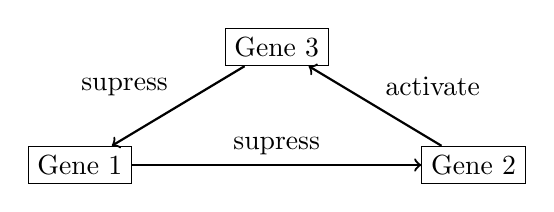
\begin{tikzpicture}
			\node (g1) at (0,0) [rectangle, draw] {Gene 1};
			\node (g2) at  (5,0) [rectangle, draw] {Gene 2}; 
			\node (g3) at (2.5, 1.5) [rectangle, draw] {Gene 3}; 
			
			\draw [thick, ->] (g1) to node [above] {supress} (g2); 
			\draw [thick, ->] (g2) to node [above right] {activate} (g3);
			\draw [thick, ->] (g3) to node [above left] {supress} (g1); 			
		\end{tikzpicture}
		\label{fig: ExGeneInteraction}
		\caption{Example for a gene interaction network. }
	\end{figure}
	\newpage
	\item Trees
	\begin{figure} [h!]
		\centering
		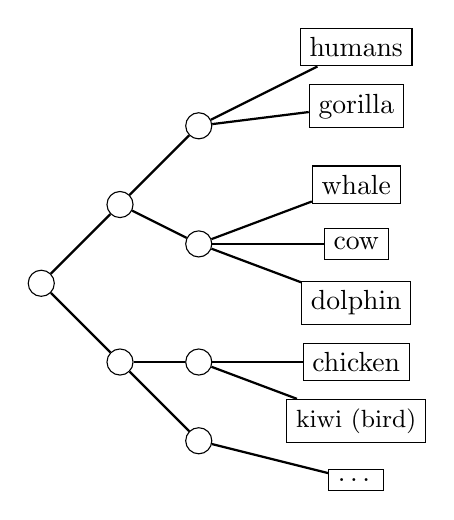
\begin{tikzpicture}
			\node (a) at (0,0) [circle, draw] []{};
			\node (aa) at (1,1) [circle, draw] {}; 
			\node (ab) at (1,-1) [circle, draw] {}; 
			\node (aaa) at (2,2) [circle, draw] {}; 
			\node (aab) at (2,0.5) [circle, draw] {}; 
			\node (aba) at (2,-1) [circle, draw] {}; 
			\node (abb) at (2,-2) [circle, draw] {}; 
			\node (aaaa) at (4,3) [rectangle, draw] {humans}; 
			\node (aaab) at (4,2.25) [rectangle, draw] {gorilla}; 
			\node (aaba) at (4,1.25) [rectangle, draw] {whale}; 
			\node (aabb) at (4,0.5) [rectangle, draw] {cow}; 
			\node (aabc) at (4,-0.25) [rectangle, draw] {dolphin}; 
			\node (abaa) at (4,-1) [rectangle, draw] {chicken}; 
			\node (abab) at (4,-1.75) [rectangle, draw] {\small 
				kiwi (bird)}; 
			\node (abba) at (4,-2.5) [rectangle, draw] {$\dots$}; 
			
			\draw [thick, -] (a) to (aa);
			\draw [thick, -] (a) to (ab);
			\draw [thick, -] (aa) to (aaa);
			\draw [thick, -] (aa) to (aab);
			\draw [thick, -] (ab) to (aba);
			\draw [thick, -] (ab) to (abb);
			\draw [thick, -] (aaa) to (aaaa);
			\draw [thick, -] (aaa) to (aaab);
			\draw [thick, -] (aab) to (aaba);
			\draw [thick, -] (aab) to (aabb);
			\draw [thick, -] (aab) to (aabc);
			\draw [thick, -] (aba) to (abaa);
			\draw [thick, -] (aba) to (abab);
			\draw [thick, -] (abb) to (abba);
		\end{tikzpicture}
		\label{fig: ExTree}
		\caption{Shortened Tree of Life as example for a tree}
	\end{figure}
	\end{itemize}
	
	$\Rightarrow $ Graph theory is an important topic in mathamatics. 
\end{eg}

\underline{Some classic results: }
\begin{defi}
	\textbf{planar graph: } \\
	Is graph G planar, i.e can it be drawn in the plane without edges crossing? 
\end{defi}
\begin{eg}
	\begin{itemize} 
		\item K(3,2): Is it posible to conect all blue nodes to all white nodes without any edges crossing?
		\begin{figure}[h!]
			\centering
			\begin{tabular}[h!]{ccc}							
		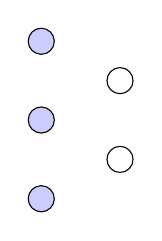
\begin{tikzpicture}
		\tikzstyle{first}=[fill=blue!20]
			\node[first] (a1) at (0,0) [circle, draw] {};
			\node[first] (a2) at (0,-1) [circle, draw] {};
			\node[first] (a3) at (0,-2) [circle, draw] {};
			\node (b1) at (1,-0.5) [circle, draw] {};
			\node (b2) at (1,-1.5) [circle, draw] {};
		\end{tikzpicture}
		& {\LARGE $\Rightarrow$ }
		&
		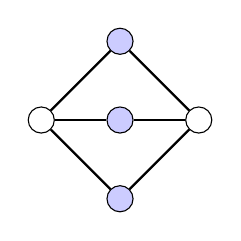
\begin{tikzpicture}
			\tikzstyle{first}=[fill=blue!20]
			\node[first] (a1) at (0,0) [circle, draw] {};
			\node[first] (a2) at (0,-1) [circle, draw] {};
			\node[first] (a3) at (0,-2) [circle, draw] {};
			\node (b1) at (1,-1) [circle, draw] {};
			\node (b2) at (-1,-1) [circle, draw] {};
			
			\draw [thick, -] (b1) to (a1);
			\draw [thick, -] (b1) to (a2);
			\draw [thick, -] (b1) to (a3);
			\draw [thick, -] (b2) to (a1);
			\draw [thick, -] (b2) to (a2);
			\draw [thick, -] (b2) to (a3);
		\end{tikzpicture}
		\\
		\end{tabular}
		\label{fig: k(3,2)-a}
		\caption{K(3,2)-problem and its solution  }
	\end{figure}

	\item K(3,3) 
	\begin{figure}[h!]
		\centering
		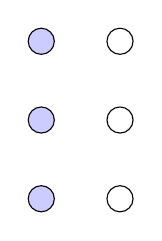
\begin{tikzpicture}
		\tikzstyle{first}=[fill=blue!20]
		\node[first] (a1) at (0,0) [circle, draw] {};
		\node[first] (a2) at (0,-1) [circle, draw] {};
		\node[first] (a3) at (0,-2) [circle, draw] {};
		\node (b1) at (1,0) [circle, draw] {};
		\node (b2) at (1,-1) [circle, draw] {};
		\node (b3) at (1, -2) [circle, draw] {}; 
		\end{tikzpicture}
		\caption{For the K(3,3)-Problem there is no posibility to connect each blue node with each white without any edges crossing}
	\end{figure}
	\\ $\Rightarrow$ K(3,3) is not planar.
	\item $K_{4}$ : connect each node out of 4 with all other nodes: 
	\begin{figure}[h!]
		\centering
		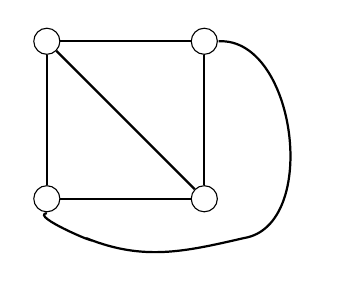
\begin{tikzpicture}
			\node (a) at (0,2) [circle, draw] {}; 
			\node (b) at (0,0) [circle, draw] {}; 
			\node (c) at (2,0) [circle, draw] {}; 
			\node (d) at (2,2) [circle, draw] {}; 
			
			\draw [thick, -] (a) to (b);
			\draw [thick, -] (a) to (c);
			\draw [thick, -] (a) to (d);
			\draw [thick, -] (b) to (c);
			\draw [thick, -] (c) to (d);
			%\draw [thick, -] (b) to (d);
			\draw [thick] (0,-0.182) % Draws a line
			to [out=189,in=334] (0.5,-0.5)
			to [out=-22,in=193] (2.5,-0.5) 
			to [out=9,in=3] (2.182,2);
		\end{tikzpicture}
		\caption{Solution for $K_{4}$}
	\end{figure}
	
	\item $K_{5} $ is not planar
	\end{itemize}
\end{eg}
\newpage
\begin{defi}
	G is planar $\Leftrightarrow$ G does not "contain" $K(3,3)$ or $K_{5}$. 
\end{defi}
\begin{eg}
	\textbf{The 4 color Theorem: } any planar given "map" can be colored in a way that no 2 countries with the same color share a comon border (edges are no borders), by only using 4 different colors. \\
	\textbf{Proof: } by using the 5 color theorem\\
	First proofed in the 70s by Kenneth Appel and Wolfgang Haken using a pascal programm called "hand-hand-hand", which handled many many cases. It was the first major thorem proofed by using a computer.  
\end{eg}
\begin{defi}
	A \textbf{undirected Grap} G(V,E) has a finite node set V and edge set E, where edge $e =  \{v,w\}$ with $v, w \in V$. \\
	v,w are \textbf{endpoints} of e and are \textbf{incident} to e. \\
	Two edges e1 and e2 $\in E$ are \textbf{adjacent}, if $e1 \cap e2 \neq 0$ i.e. they share a node. 
\end{defi}
\begin{defi}
	The \textbf{degree} of a node d(v) = $| \{e \in E | v \in e \} |$\\
	($\#$ of edges of v)
	\begin{figure}[h!]
		\centering
		
		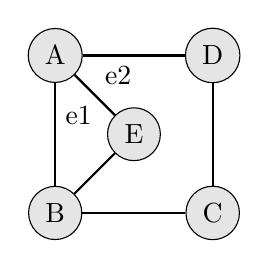
\begin{tikzpicture}
		\tikzstyle{first}=[fill=gray!20]
		\node[first] (b) at (0,0) [circle, draw] {B};
		\node[first] (a) at (0,2) [circle, draw] {A};
		\node[first] (d) at (2,2) [circle, draw] {D};
		\node[first] (c) at (2,0) [circle, draw] {C};
		\node[first] (e) at (1,1) [circle, draw] {E};
		
		\draw [thick, -] (a) to (d);
		\draw [thick, -] (a) to node [above right] {e1} (b);
		\draw [thick, -] (a) to node [above right] {e2} (e);
		\draw [thick, -] (d) to (c);
		\draw [thick, -] (b) to (e);
		\draw [thick, -] (b) to (c);
		\end{tikzpicture}
		\caption{\textbf{Example to Definition 1.5: }d(a)= 3; e1, e2 are incident to e and e1, e2 are adjacent}
	\end{figure}
	
	We will usually assume: 
	\begin{enumerate}
		\item $|\{e\}| = 2$, i.e. no self-loops 
		\begin{figure}[h!]
			\centering
			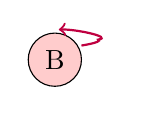
\begin{tikzpicture}
				\tikzstyle{first}=[fill=red!20]
				\node[first] (b) at (0,0) [circle, draw] {B}; 
				\draw [thick,purple, ->]  (0.35,0.182) % Draws a line
				to [out=189,in=334] (0.55,0.255)
				to [out=9,in=3] (0.05,0.382);
			\end{tikzpicture}
		\end{figure}
		\item all edges are different 
		\begin{figure}[h!]
			\centering
			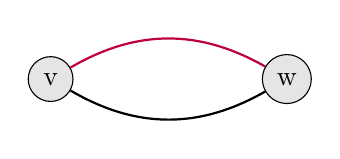
\begin{tikzpicture}
			\tikzstyle{first}=[fill=gray!20]
			\node [first] (a) at (0,0) [circle, draw] {v}; 
			\node[first] (b) at (3,0) [circle, draw] {w}; 
			\draw [thick,-] (a) to [bend right](b);
			\draw [thick,purple, -] (b) to [bend right](a);
			\end{tikzpicture}
		\end{figure}
	\end{enumerate}
\end{defi}
\begin{defi}
	A \textbf{directed graph} G = (V,E) has a node set V and edge set E, with e = (V, W) = (source node, taget node)\\
	Like to draw this: 
	\begin{figure}[h!]
		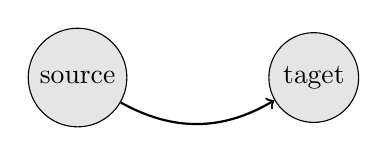
\begin{tikzpicture}
			\tikzstyle{first}=[fill=gray!20]
			\node [first] (a) at (0,0) [circle, draw] {source}; 
			\node[first] (b) at (3,0) [circle, draw] {taget}; 
			\draw [thick,->] (a) to [bend right](b);
		\end{tikzpicture}
	\end{figure}
\end{defi}
\newpage
\begin{defi}
    . 
	\begin{itemize}
		\item \textbf{Indegree:} Indeg(v) = $|\{(w,v) \in E\}|$ \\
		$\#$ of all edges that go into the node. 
		\item \textbf{Outdegree:} Outdeg(v) = $|\{(v,w) \in E\}|$ \\
		$\#$ of all edges that go out of the node.
		\item \textbf{Degree: } Deg(v) = Indeg(v) + Outdeg(v)
	\end{itemize}
\end{defi}

\subsection{Implementing a graph}
\begin{enumerate}
	\item Implement directed graph then add return edges
	\begin{figure}[h!]
		\centering
		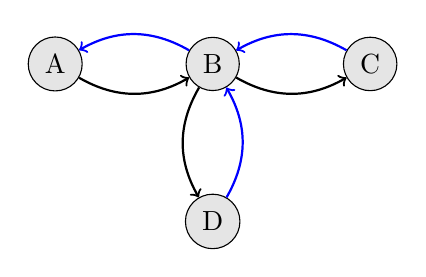
\begin{tikzpicture}
			\tikzstyle{first}=[fill=gray!20]
			\node [first] (a) at (0,0) [circle, draw] {A}; 
			\node [first] (b) at (2,0) [circle, draw] {B}; 
			\node [first] (c) at (4,0) [circle, draw] {C};
			\node [first] (d) at (2,-2) [circle, draw] {D};  
			
			\draw [thick,->] (a) to [bend right](b);
			\draw [thick,->] (b) to [bend right](c);
			\draw [thick,->] (b) to [bend right](d);
			\draw [thick,blue,->] (b) to [bend right](a);
			\draw [thick,blue,->] (c) to [bend right](b);
			\draw [thick,blue,->] (d) to [bend right](b);
		\end{tikzpicture}
		\caption{D (black) Graph. U (black $\&$ blue) extends Graph D}
	\end{figure}
\end{enumerate}
Note: source and taget does not matter in undirected graphs. 
\begin{defi}
	Let $G^{*} = (V^{*},E^{*})$, subgraph of G = (V,E), if $V^{*} \subseteq V$ and $E^{*} \subseteq E $ with $E^{*} \subseteq V^{*}xV^{*}$
\end{defi}
\begin{defi}
	An \textbf{Euleianr-tour (path)} describes an path on a given graph G where every edge is visited just once. An eulerian path exists iff (=if and only if) the number of nodes with odd degrees is 0 or 2. 
	\begin{figure}[h!]
		\centering
		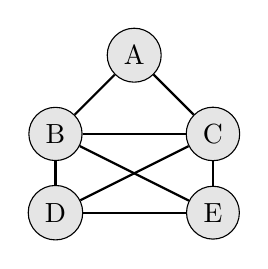
\begin{tikzpicture}
			\tikzstyle{first}=[fill=gray!20]
			\node [first] (a) at (2,3) [circle, draw] {A}; 
			\node[first] (b) at (1,2) [circle, draw] {B}; 
			\node[first] (c) at (3,2) [circle, draw] {C}; 
			\node[first] (d) at (1,1) [circle, draw] {D}; 
			\node[first] (e) at (3,1) [circle, draw] {E}; 
			\draw [thick,-] (a) to (b);
			\draw [thick,-] (a) to (c);
			\draw [thick,-] (b) to (d);
			\draw [thick,-] (b) to (c);
			\draw [thick,-] (b) to (e);
			\draw [thick,-] (c) to (e);
			\draw [thick,-] (c) to (d);
			\draw [thick,-] (e) to (d);
		\end{tikzpicture}
		\caption{Example for an Eulerian path: Only D and E have a odd number auf edges. So there exists an eulerian tour in this graph.}
	\end{figure}
\end{defi}
\begin{defi}
	Let G = (V,E) be a (directed or undirected) graph. A \textbf{subgraph} G' = (V',E') of G is a graph whose node and edges sets are subsets of those of G, that is, V' $\subseteq$ V and E' $\subseteq$ E, such that the edges in E' only contain nodes in V'. \\
	Let $U \subseteq V$. The subgraph $G|_U = (U, E|_U)$ \textbf{induced } by U has node set U and induced edge set $E|_U$ consisting of all edges in G whose endpoints both lie in U. 
	\begin{figure}[h!]
		\centering
		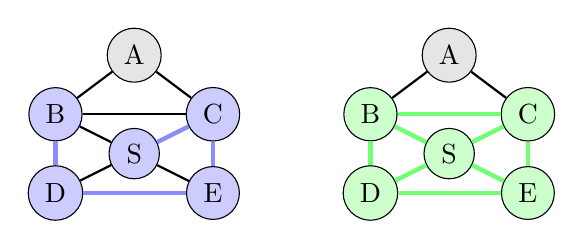
\begin{tikzpicture}
		\tikzstyle{first}=[fill=gray!20]
		\tikzstyle{subset}=[fill=blue!20]
		\tikzstyle{induced}=[fill=green!20]
		%%%%%%%%%%%%%%%%%%%%%left subgraph %%%%%%%%%%%%%%%%%%%
		\node [first] (a) at (2,2.75) [circle, draw] {A}; 
		\node[subset] (b) at (1,2) [circle, draw] {B}; 
		\node[subset] (c) at (3,2) [circle, draw] {C};
		\node [subset] (s) at (2, 1.5) [circle, draw] {S};  
		\node[subset] (d) at (1,1) [circle, draw] {D}; 
		\node[subset] (e) at (3,1) [circle, draw] {E}; 
		\draw [thick,-] (a) to (b);
		\draw [thick,-] (a) to (c);
		\draw [ultra thick, blue!45,-] (b) to (d);
		\draw [thick,-] (b) to (c);
		\draw [thick,-] (b) to (s);
		\draw [ultra thick, blue!45,-] (c) to (e);
		\draw [ultra thick, blue!45,-] (c) to (s);
		\draw [ultra thick, blue!45,-] (e) to (d);
		\draw [thick,-] (e) to (s);
		\draw [thick,-] (d) to (s);
		%%%%%%%%%%%%%%%%%%%%%right subgraph %%%%%%%%%%%%%%%%%%%
		\node [first] (a1) at (6,2.75) [circle, draw] {A}; 
		\node[induced] (b1) at (5,2) [circle, draw] {B}; 
		\node[induced] (c1) at (7,2) [circle, draw] {C};
		\node [induced] (s1) at (6, 1.5) [circle, draw] {S};  
		\node[induced] (d1) at (5,1) [circle, draw] {D}; 
		\node[induced] (e1) at (7,1) [circle, draw] {E}; 
		\draw [thick,-] (a1) to (b1);
		\draw [thick,-] (a1) to (c1);
		\draw [ultra thick, green!55,-] (b1) to (d1);
		\draw [ultra thick, green!55,-] (b1) to (c1);
		\draw [ultra thick, green!55,-] (b1) to (s1);
		\draw [ultra thick, green!55,-] (c1) to (e1);
		\draw [ultra thick, green!55,-] (c1) to (s1);
		\draw [ultra thick, green!55,-] (e1) to (d1);
		\draw [ultra thick, green!55,-] (e1) to (s1);
		\draw [ultra thick, green!55,-] (d1) to (s1);
		\end{tikzpicture}
		\caption{Example for subgraph (blue) of G (black) and an induced subgraph (green) of G.}
	\end{figure}
\end{defi}
\begin{defi}
	Let G=(V,E) be a graph. A \textbf{undirected path} in G is defined as: p($v_0, e_1, v_1, e_2, v_2, \dots e_k, v_k$) with $v_i \in V$, $e_i \in E$ and $e_i =\{v_{i-1}, v_i\}$ and $e_i \neq e_j \forall i \neq j$. \\
	p \textbf{connects} $v_0$ to $v_k$. If $v_0 = v_k$, then p is called a \textbf{cycle}. \\
	If G is directed, then p is directed if $e_i = (v_{i-1}, v_i)$\\
	A undirected Graph G = (V,E) is \textbf{connected}, if $\forall v,w \in V: \exists $ path p form v to w. \\
	A directed graph G = (V,E) is \textbf{(weakly) connected} if any two nodes are connected by an undirected path. G is called \textbf{(strongly) connected}, if there is a directed path from v to w and a directed path from w to v. 
	
	\begin{figure}[h!]
		\centering
		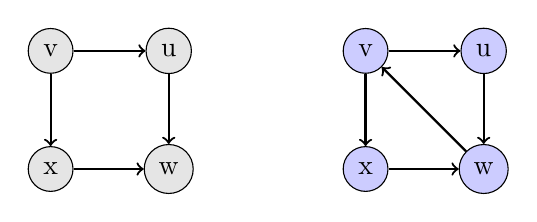
\begin{tikzpicture}
			\tikzstyle{first}=[fill=gray!20]
			\tikzstyle{second}=[fill=blue!20]
			\node [first] (v) at (0,1.5) [circle, draw] {v}; 
			\node [first] (x) at (0,0) [circle, draw] {x}; 
			\node [first] (u) at (1.5,1.5) [circle, draw] {u}; 
			\node [first] (w) at (1.5,0) [circle, draw] {w}; 
			
			\draw [thick, ->] (v) to (u);
			\draw [thick, ->] (v) to (x);
			\draw [thick, ->] (x) to (w);
			\draw [thick, ->] (u) to (w);
			
			% 2. subgraph 
			\node [second] (v1) at (4,1.5) [circle, draw] {v}; 
			\node [second] (x1) at (4,0) [circle, draw] {x}; 
			\node [second] (u1) at (5.5,1.5) [circle, draw] {u}; 
			\node [second] (w1) at (5.5,0) [circle, draw] {w}; 
			
			\draw [thick, ->] (v1) to (u1);
			\draw [thick, ->] (v1) to (x1);
			\draw [thick, ->] (x1) to (w1);
			\draw [thick, ->] (u1) to (w1);
			\draw [thick, ->] (w1) to (v1); 
		\end{tikzpicture}
		\caption{Example for connected graphs: The gray graph is weakly connected, while the blue graph is strongly connected.}
	\end{figure}
\end{defi}
\begin{eg}
	\textbf{The Chinese Postman theorem: }
	The postman searches for the best tour to deliver the mail. He wants to visit each edge once in a tour and minimize the edges. 
	
	\begin{figure} [h!]
		\centering
		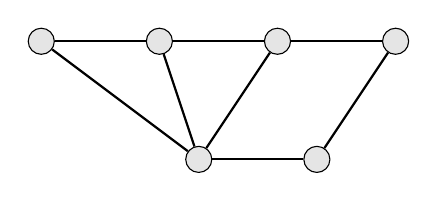
\begin{tikzpicture}
		\tikzstyle{first}=[fill=gray!20]
		\node[first](a) at (0,3) [circle, draw] {}; 
		\node[first](b) at (1.5,3) [circle, draw] {}; 
		\node[first](c) at (3,3) [circle, draw] {}; 
		\node[first](d) at (4.5,3) [circle, draw] {}; 
		\node[first](e) at (2,1.5) [circle, draw] {}; 
		\node[first](f) at (3.5,1.5) [circle, draw] {}; 
		
		\draw [thick, -] (a) to (b);
		\draw [thick, -] (a) to (e);
		\draw [thick, -] (b) to (e);
		\draw [thick, -] (b) to (c);
		\draw [thick, -] (c) to (e);
		\draw [thick, -] (c) to (d);
		\draw [thick, -] (d) to (f);
		\draw [thick, -] (f) to (e);
		\end{tikzpicture}
		\caption{Example of a posible map for the postman theorem}
	\end{figure}
	$\Rightarrow$
	Is the graph undirected, an optimal tour can be planed in polynominal time. \\
	Is the graph directed, again an optimal tour can be planed in polynominal time. \\
	But if the graph is both (directed and undirected), then the problem is NP hard. 
\end{eg}
\subsection {Trees}
\begin{defi}
	A \textbf{directed acyclic graph (DAG)} is a directed graph with noch directed cycles. 
	
	\begin{figure}[h!]
		\centering
		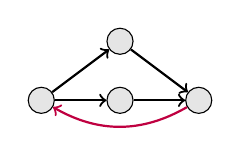
\begin{tikzpicture}
			\tikzstyle{first}=[fill=gray!20]
			\node[first](a) at (0,2) [circle, draw] {}; 
			\node[first](b) at (1,2) [circle, draw] {}; 
			\node[first](c) at (1,2.75) [circle, draw] {}; 
			\node[first](d) at (2,2) [circle, draw] {};
			
			\draw [thick, ->] (a) to (b);
			\draw [thick, ->] (a) to (c);
			\draw [thick, ->] (b) to (d);
			\draw [thick, ->] (c) to (d);
			\draw [thick, purple, ->] (d) to [bend left](a);
		\end{tikzpicture}
		\caption{This graph showes a graph, without the red path this graph is a DAG, with the red path a cycle exists.}
	\end{figure} 
\end{defi}

\begin{defi}
	A \textbf{Tree} is a connected graph with no undirected cycles.
	\begin{figure} [h!]
		\centering
		\begin{tabular}{c|c}
		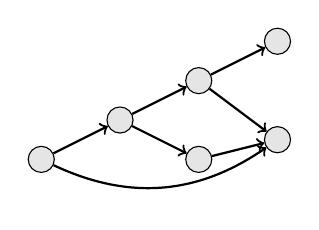
\begin{tikzpicture}
			\tikzstyle{first}=[fill=gray!20]
			\node[first](a) at (0,0) [circle, draw] {};
			\node[first](b) at (1,0.5) [circle, draw] {};
			\node[first](c) at (2,1) [circle, draw] {};
			\node[first](d) at (3,1.5) [circle, draw] {};
			\node[first](e) at (2,0) [circle, draw] {};
			\node[first](f) at (3,0.25) [circle, draw] {};
			
			\draw [thick, ->] (a) to (b);
			\draw [thick, ->] (b) to (c);
			\draw [thick, ->] (b) to (e);
			\draw [thick, ->] (c) to (d);
			\draw [thick, ->] (c) to (f);
			\draw [thick, ->] (e) to (f);
			\draw [thick, ->] (a) to [bend right] (f);
		\end{tikzpicture}
	&
	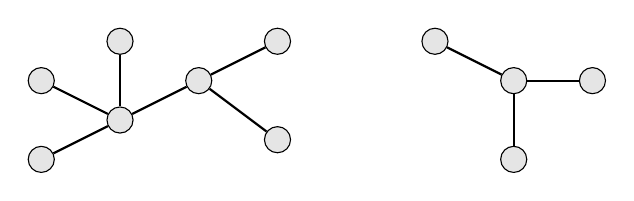
\begin{tikzpicture}
		\tikzstyle{first}=[fill=gray!20]
		\node[first](a) at (0,0) [circle, draw] {};
		\node[first](b) at (1,0.5) [circle, draw] {};
		\node[first](c) at (2,1) [circle, draw] {};
		\node[first](d) at (3,1.5) [circle, draw] {};
		\node[first](e) at (1,1.5) [circle, draw] {};
		\node[first](f) at (3,0.25) [circle, draw] {};
		\node[first](aa) at (0,1) [circle, draw] {};
		
		\draw [thick, -] (a) to (b);
		\draw [thick, -] (aa) to (b);
		\draw [thick, -] (e) to (b);
		\draw [thick, -] (b) to (c);
		\draw [thick, -] (c) to (d);
		\draw [thick, -] (c) to (f);
		
		\node[first](a1) at (6,1) [circle, draw] {};
		\node[first](a2) at (6,0) [circle, draw] {};
		\node[first](a3) at (7,1) [circle, draw] {};
		\node[first](a4) at (5,1.5) [circle, draw] {};
		
		\draw [thick, -] (a1) to (a2);
		\draw [thick, -] (a3) to (a1);
		\draw [thick, -] (a4) to (a1);
		
	\end{tikzpicture}
	\\
	This graph is not a (rooted) tree. 
	&
	This graph consists out of several unrooted trees and is called a \textbf{forest}. 	
	\end{tabular}
	\end{figure} 
	Any such tree is called \textbf{unrooted}. \\
	In a \textbf{rooted tree} exactly one (!one) node $\zeta \in V$ is declared \textbf{root} and we write T = (V, E, $\zeta$). \\
	We can consider a rooted tree als directed graph, by directing all edges away from the root. 	
	\begin{figure} [h!]
		\centering
		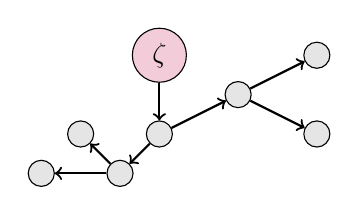
\begin{tikzpicture}
			\tikzstyle{first}=[fill=gray!20]
			\tikzstyle{root}=[fill=purple!20]
			\node[first](a) at (0.5,0) [circle, draw] {};
			\node[first](b) at (1,0.5) [circle, draw] {};
			\node[first](c) at (2,1) [circle, draw] {};
			\node[first](d) at (3,1.5) [circle, draw] {};
			\node[root](e) at (1,1.5) [circle, draw] {$\zeta$};
			\node[first](f) at (3,0.5) [circle, draw] {};
			\node[first](aa) at (0,0.5) [circle, draw] {};
			\node[first](bl) at (-0.5,0) [circle, draw] {};
			
			\draw [thick, ->] (b) to (a);
			\draw [thick, ->] (a) to (aa);
			\draw [thick, ->] (e) to (b);
			\draw [thick, ->] (b) to (c);
			\draw [thick, ->] (c) to (d);
			\draw [thick, ->] (c) to (f);
			\draw [thick, ->] (a) to (bl); 
		\end{tikzpicture}
		\caption{Example for Def 1.13: all edges are directed away from the root $\zeta$.}
	\end{figure}
\end{defi}
% TOOD add examples of how different Trees are drawn in computer science, biology ect
\begin{defi}.
	\newline
	In an \underline{unrooted tree}: nodes of degree 1 are called \textbf{leaf}. \newline
	In a \underline{rooted tree}: nodes of outdegree 0 are called \textbf{leaf}. \newline
	All other nodes are called \textbf{internal nodes}. 
\end{defi}
\begin{defi}
	For a \underline{rooted tree} :
	\begin{itemize}
		\item there has to be one node with indegree 0, the root 
		\item The tree is called \textbf{biforcation (binary, fully resolved)} if each internal node has degree 3\\
		(In directed rooted tree: indegree 1, outdegree 2)\\
		and \textbf{multiforcation}, else. 
		
	\end{itemize} 
	
	\begin{figure}[h!]
		\centering
		\begin{tabular}{cc|cc}
			biforcation &&& multiforcation\\
			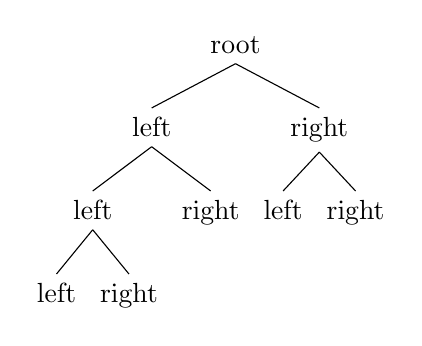
\begin{tikzpicture}
				\Tree[.root [.left [.left left right ] right ] [.right left right ] ];		
			\end{tikzpicture}
			&&&
			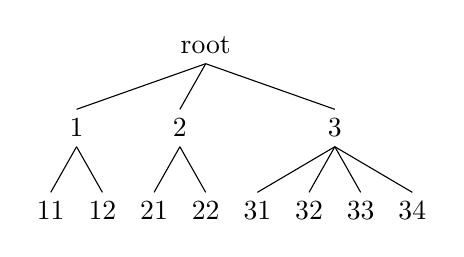
\begin{tikzpicture}
				\Tree[.root [.1 11 12 ] [.2 21 22 ] [.3 31 32 33 34 ] ];
			\end{tikzpicture}
			\\
		\end{tabular}
		\caption{example trees for biforcation and multiforcation}
	\end{figure}
\end{defi}

\begin{defi}
	Let T rooted tree and $v \in V$ node in T. A \textbf{subtree} $T_v$  \underline{rooted } at v looks like this: \\
	\begin{figure}[h!]
		\begin{tabular}{ccc|ccc}
			tree T: 
			&
			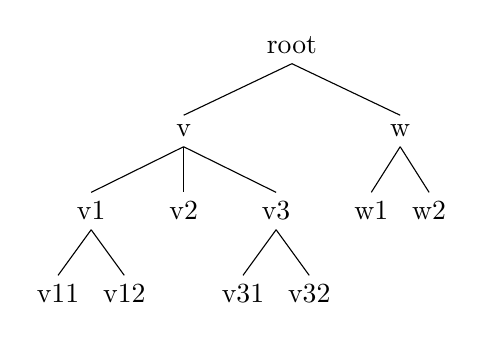
\begin{tikzpicture}
				\Tree[.root [.v [.v1 v11 v12 ] v2 [.v3 v31 v32 ] ] [.w w1 w2 ] ]
			\end{tikzpicture}
			&&& 
			subtree $T_v$			
			&
			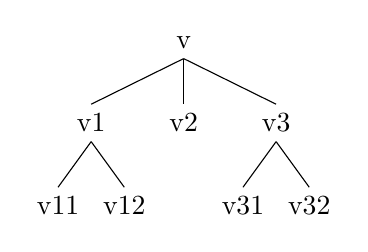
\begin{tikzpicture}
				\Tree[.v [.v1 v11 v12 ] v2 [.v3 v31 v32 ] ]
			\end{tikzpicture}
			\\
		\end{tabular}
	\end{figure}
	$T_v$ is tree with root v that is \textbf{induced by v} and all nodes reachable from v by a directed path starting at v. 
\end{defi}

\subsection{Tree traversals}
For the following algorithms let T be a biforcating rooted tree (compare figure 17)\\
(The algorithms run analog for multiforcation trees)
	\begin{figure}[h!] 
		\centering
		\begin{tikzpicture} [sibling distance=13pt]
		\Tree[.$\zeta$ [.j [.h [.g a b ] c ] e ] f ]
		\end{tikzpicture}
		\caption{We will use this tree T for all traversals }
	\end{figure}
\begin{itemize}
	\item \textbf{Pre-order traversal (top down)} \\
	\textit{Examine (e.g. print out a lable) the root of T\\
		Traverse \underline{left} subtree\\
		Travers \underline{right} subtree} \\
	\textbf{Result on tree T:} $ \zeta, j, h, g, a, b, c, i, d, e, f$ \\
	(Algoritmic representation: root, traverse $T_j$, traverse $T_f$)

	\item \textbf{Post-order traversal (bottom up)} \\
	\textit{Traverse \underline{left} subtree\\
		Travers \underline{right} subtree\\
			Examine} \\		
	\textbf{Result on tree T:} $ a, b, g, c, h, d, e, i, j, f, \zeta$ \\
		
	\item \textbf{Inorder traversal } \\
	\textit{Traverse \underline{left} subtree,\\
		Examine,\\
		Travers \underline{right} subtree
		} \\		
	\textbf{Result on tree T:} $ f, \zeta, e, j, c, h, b, g, a$ \\
	Extention for multification trees: Sometimes it might be required to examine the root between several children. 
	
	\item \textbf{Break first } \\
	\textit{Put root $\zeta$ in a queue\\
		While queue not empty\\
		Pop off queue\\
		Examine\\
		Add children to end of queue}\\
	\textbf{Result on tree T: }
	\begin{tabular}{lll}
		& Q:= $\zeta$ & v $\leftarrow \zeta$ \\
		v: $\zeta$ & Q = (j, f) & v $\leftarrow$ j\\
		v: j & Q = (f, h, i) & v $\leftarrow$ f \\
		v: f & Q = (h, i) & v $\leftarrow$  h \\
		v: h & Q = (i, g, c) & v $\leftarrow$ i \\
		v: i & Q = (g, c, d, e) & v $\leftarrow$ g \\
		v: g & Q = (c, d, e, a, b) & v $\leftarrow$ c\\
		v: c & Q = (d, e, a, b) & \dots \\
		v: d & Q = (e, a, b) & \\
		v: e & Q = (a, b) &\\
		v: a & Q = (b) &\\
		v: b & Q = () & \\ 	
	\end{tabular}
	\\The first row of the tabular represents the order in which the nodes where examined. \\
	Proof: Quque higher level $\rightarrow$ first in quque. 	
	
	\item Pre-, post- and Inorder traversal are \textbf{depth first traversals}. 
\end{itemize}


\newpage
\section{References}
\subsection{Figures}
\begin{tabular}[h] {rrr}
 Figure  & Source & time\\
 \hline
Figure \ref{fig:foodweb} & \url{http:////mdk12.msde.maryland.gov//instruction//clg//public\_release//biology//g3\_e5\_i2.html}  & 2015-10 \\
\end{tabular}
\end{document}